\section{Estimator and Training-Period-Frozen Analysis-Domain Sensitivity}
\label{supsec:estimator_domain}

The E09 sensitivity analysis evaluated the plug-in, Miller--Madow, and
coherent observed-support Jeffreys--Dirichlet estimators across 16
prespecified specifications in each city. All 16 DELB-reduction point
estimates were positive for every city and estimator
(Table~\ref{tab:sup_estimator_specifications}). The Jeffreys calculation
places a symmetric posterior on observed full-joint atoms and coherently
aggregates its marginals; it does not reconstruct unobserved support.

E17 applied all three estimators to the same 999 temporal-block, spatial-series,
and circular-shift surrogates. Table~\ref{tab:sup_estimator_nulls} reports
both Benjamini--Hochberg adjustment within each estimator's nine
city--design comparisons and global adjustment over all 27 comparisons.
Figure~\ref{fig:sup_estimator_nulls} shows observed CMI relative to the
estimator-specific null mean.

\begin{table}[!htbp]
\caption{Sparse-entropy estimator sensitivity. Positive specifications are counted among the 16 prespecified designs for each city--estimator pair.}
\label{tab:sup_estimator_specifications}
\centering
\footnotesize
\begin{tabular*}{\linewidth}{@{\extracolsep{\fill}}llrrr@{}}
\toprule
\textbf{City} & \textbf{Estimator} & \textbf{Positive specs} & \textbf{Primary CMI (bits)} & \textbf{Primary $\Delta L$}\\
\midrule
Washington, DC & Jeffreys--Dirichlet & 16/16 & 0.0690 & 0.0187\\
Washington, DC & Miller--Madow & 16/16 & 0.0432 & 0.0123\\
Washington, DC & Plug-in & 16/16 & 0.0526 & 0.0141\\
New York City & Jeffreys--Dirichlet & 16/16 & 0.1603 & 0.0624\\
New York City & Miller--Madow & 16/16 & 0.1314 & 0.0604\\
New York City & Plug-in & 16/16 & 0.1394 & 0.0550\\
Vancouver & Jeffreys--Dirichlet & 16/16 & 0.1904 & 0.0940\\
Vancouver & Miller--Madow & 16/16 & 0.1423 & 0.0919\\
Vancouver & Plug-in & 16/16 & 0.1597 & 0.0844\\
\bottomrule
\end{tabular*}
\end{table}


\begin{table}[!htbp]
\caption{E17 city-level estimator-specific randomization calibration. Ranges cover nine city--null-design comparisons per estimator; the final column gives rejection counts under the within-estimator nine-test and global 27-test corrections.}
\label{tab:sup_estimator_nulls}
\centering
\footnotesize
\begin{tabular}{lrrrrr}
\toprule
\textbf{Estimator} & \textbf{Observed - null mean} & \textbf{Raw $p$} & \textbf{Min. $q_9$} & \textbf{Min. $q_{27}$} & \textbf{Rejections}\\
\midrule
Jeffreys--Dirichlet & [-0.0536, -0.0016] & [0.984, 1.000] & 1.000 & 1.000 & 0/0\\
Miller--Madow & [-0.0423, -0.0012] & [0.903, 1.000] & 1.000 & 1.000 & 0/0\\
Plug-in & [-0.0470, -0.0012] & [0.980, 1.000] & 1.000 & 1.000 & 0/0\\
\bottomrule
\end{tabular}
\end{table}


\begin{figure}[!htbp]
\centering
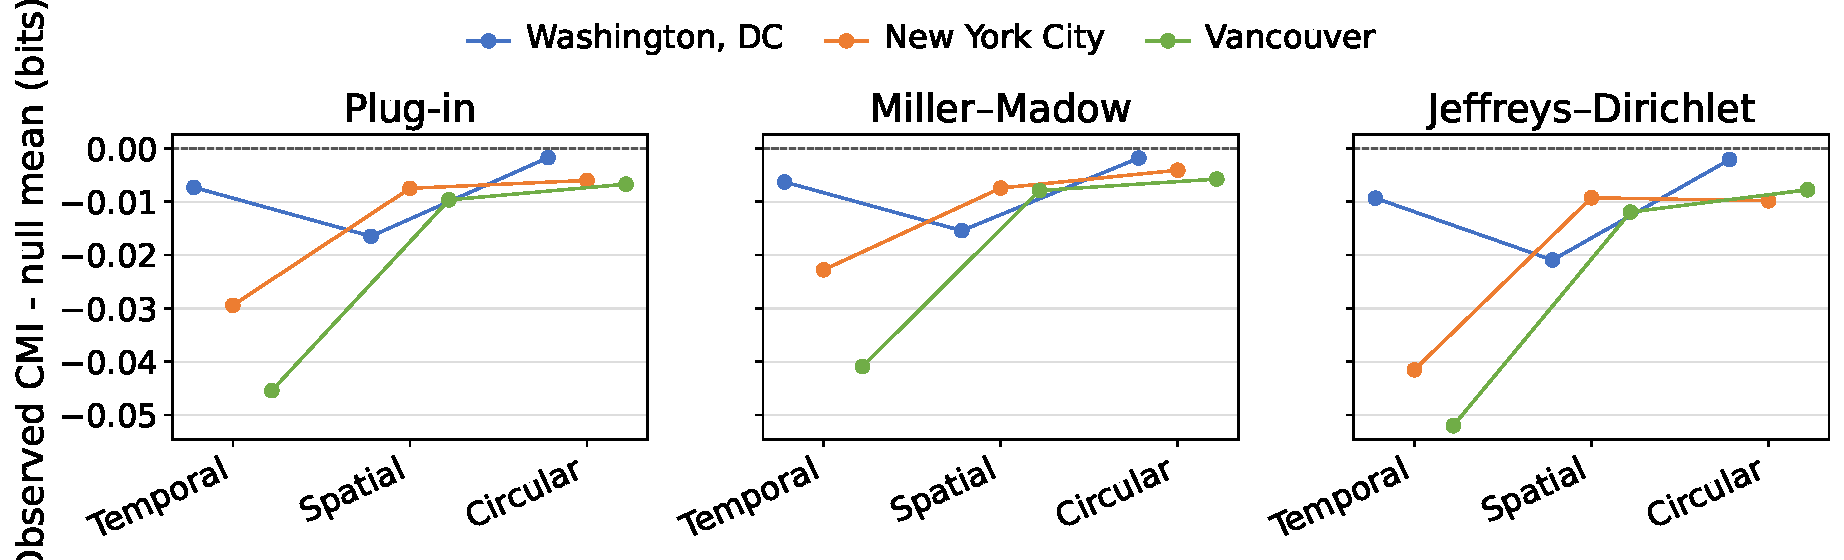
\includegraphics[width=\textwidth]{figures/e17/e17_estimator_null_sensitivity.pdf}
\caption{Estimator sensitivity of city-level randomization calibration.
Each point is the observed CMI minus the mean of the same design-conditioned
reference distribution. Nonzero null centers are allowed.}
\label{fig:sup_estimator_nulls}
\end{figure}

The analysis-domain sensitivity compares the training-period-frozen bicycle
service domain with the complete training crime-supported domain. The
domain is fixed before validation and testing; this is therefore an
analysis-population sensitivity, not a post-outcome spatial selection.
Table~\ref{tab:sup_frozen_domain} and
Figure~\ref{fig:sup_frozen_domain} show that expanding the spatial
population changes the magnitude of CMI and DELB reduction, especially in
New York City and Vancouver. These differences are descriptive and do not
identify a bicycle effect.

\begin{table}[!htbp]
\begin{adjustwidth}{-\extralength}{0cm}
\caption{Training-period-frozen analysis-domain sensitivity. Both spatial populations were defined before validation and testing.}
\label{tab:sup_frozen_domain}
\centering
\scriptsize
\setlength{\tabcolsep}{3pt}
\begin{tabular}{llrrrrrrr}
\toprule
\textbf{City} & \textbf{Analysis domain} & \textbf{Grids} & \textbf{$N$} & \textbf{CMI} & \textbf{$L^0$} & \textbf{$L^B$} & \textbf{$\Delta L$} & \textbf{Relative}\\
\midrule
Washington, DC & Frozen bicycle-covered domain & 181 & 198195 & 0.0432 & 0.1567 & 0.1443 & 0.0123 & 7.9\%\\
Washington, DC & Complete crime-supported domain & 186 & 203670 & 0.0420 & 0.1535 & 0.1416 & 0.0119 & 7.7\%\\
New York City & Frozen bicycle-covered domain & 198 & 216810 & 0.1314 & 0.3503 & 0.2898 & 0.0604 & 17.3\%\\
New York City & Complete crime-supported domain & 806 & 882570 & 0.0348 & 0.1382 & 0.1288 & 0.0094 & 6.8\%\\
Vancouver & Frozen bicycle-covered domain & 34 & 37230 & 0.1423 & 0.5113 & 0.4194 & 0.0919 & 18.0\%\\
Vancouver & Complete crime-supported domain & 141 & 154395 & 0.0377 & 0.1774 & 0.1659 & 0.0115 & 6.5\%\\
\bottomrule
\end{tabular}
\end{adjustwidth}
\end{table}


\begin{figure}[!htbp]
\centering
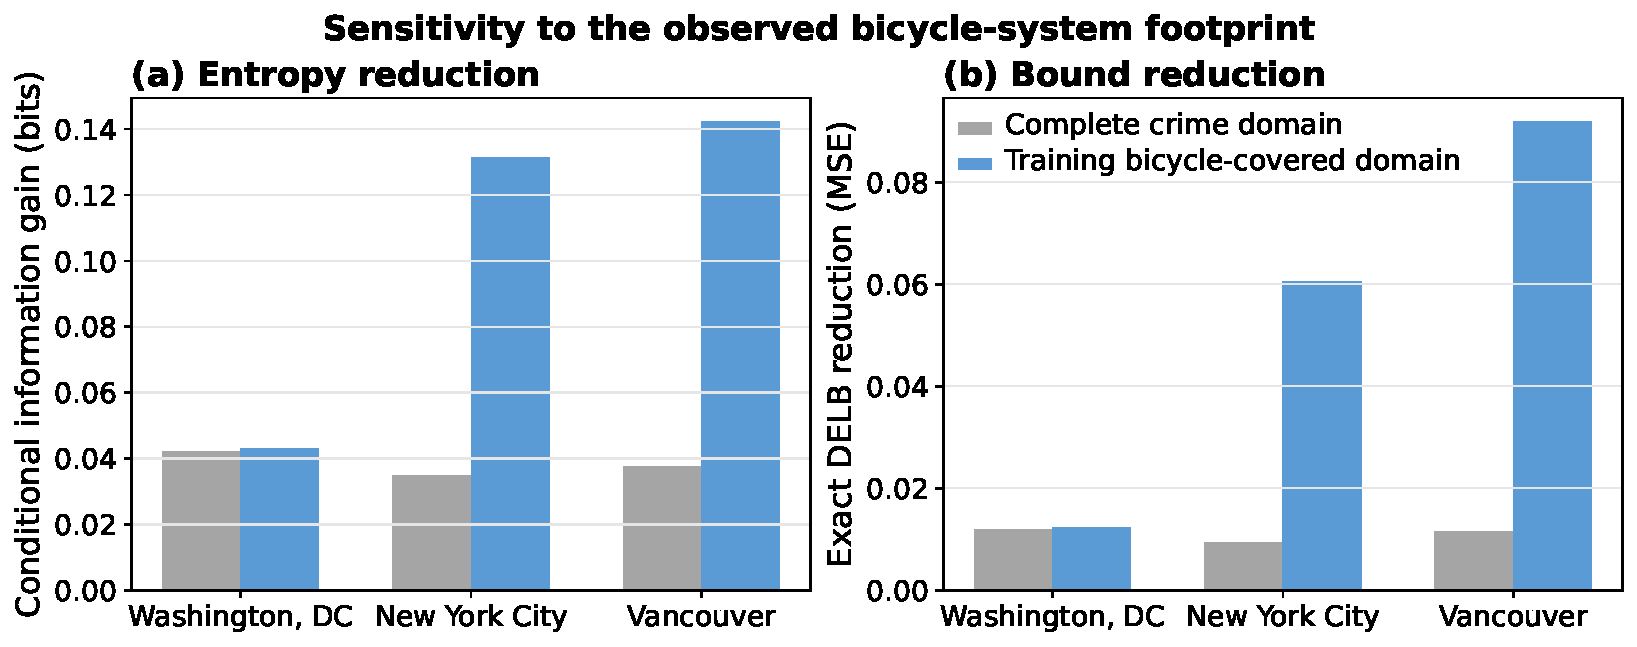
\includegraphics[width=\textwidth]{figures/e17/e04_domain_sensitivity.pdf}
\caption{Training-period-frozen analysis-domain sensitivity. The complete
crime-supported domain and the training bicycle-covered domain define
different spatial target populations.}
\label{fig:sup_frozen_domain}
\end{figure}

\section{Local Estimates and Lag-Specificity Details}
\label{supsec:moved_local_lag}


\begin{table}[H]
\caption{Spatially localized information value. The final column gives global Moran's \(I\) for DELB reduction with two-sided permutation \(p\)-values in parentheses.}
\label{tab:local_information_results}
\centering
\resizebox{\textwidth}{!}{%
\begin{tabular}{lrrrrrr}
\toprule
\textbf{City} & \textbf{Eligible/Covered} & \textbf{Median CMI} &
\textbf{Median \(\Delta L\)} & \textbf{Median \(R^L\)} &
\textbf{Positive screen} & \textbf{Moran's \(I\) (\(p\))}\\
\midrule
Washington, DC & 146/181 & 0.042 & 0.013 & 9.6\% & 137/146 & 0.164 (0.002)\\
New York City & 160/198 & 0.093 & 0.050 & 14.3\% & 155/160 & 0.038 (0.261)\\
Vancouver & 33/34 & 0.138 & 0.094 & 17.4\% & 33/33 & 0.171 (0.022)\\
\bottomrule
\end{tabular}
}
\end{table}


\begin{figure}[!htbp]
\begin{adjustwidth}{-\extralength}{0cm}
\centering
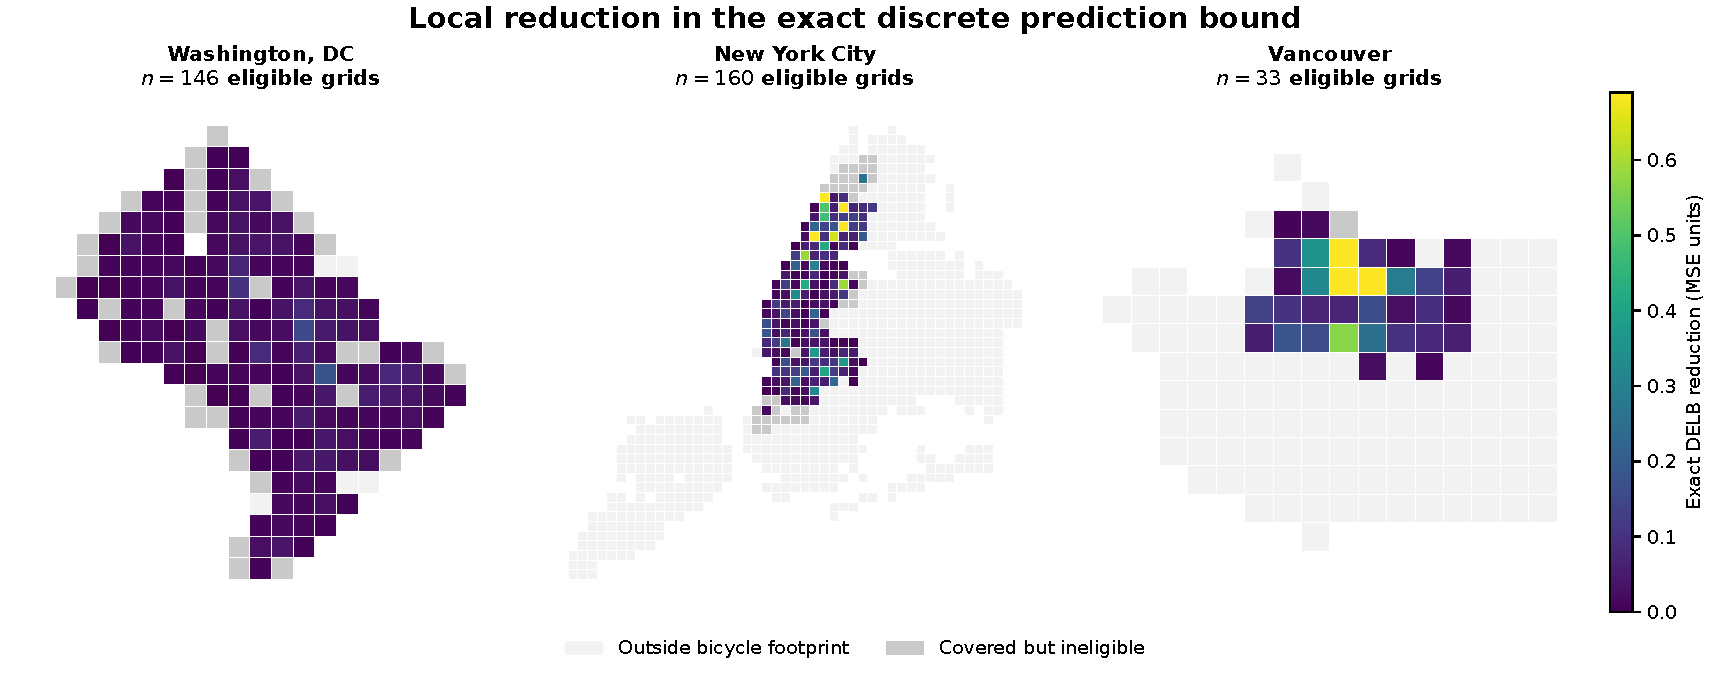
\includegraphics[width=\linewidth]{figures/e11/e05_local_delb_reduction_maps.pdf}
\end{adjustwidth}
\caption{Local DELB-reduction point estimates for eligible cells. None
passed all three randomization references.}
\label{fig:local_delb_maps}
\end{figure}

\begin{figure}[!htbp]
\centering
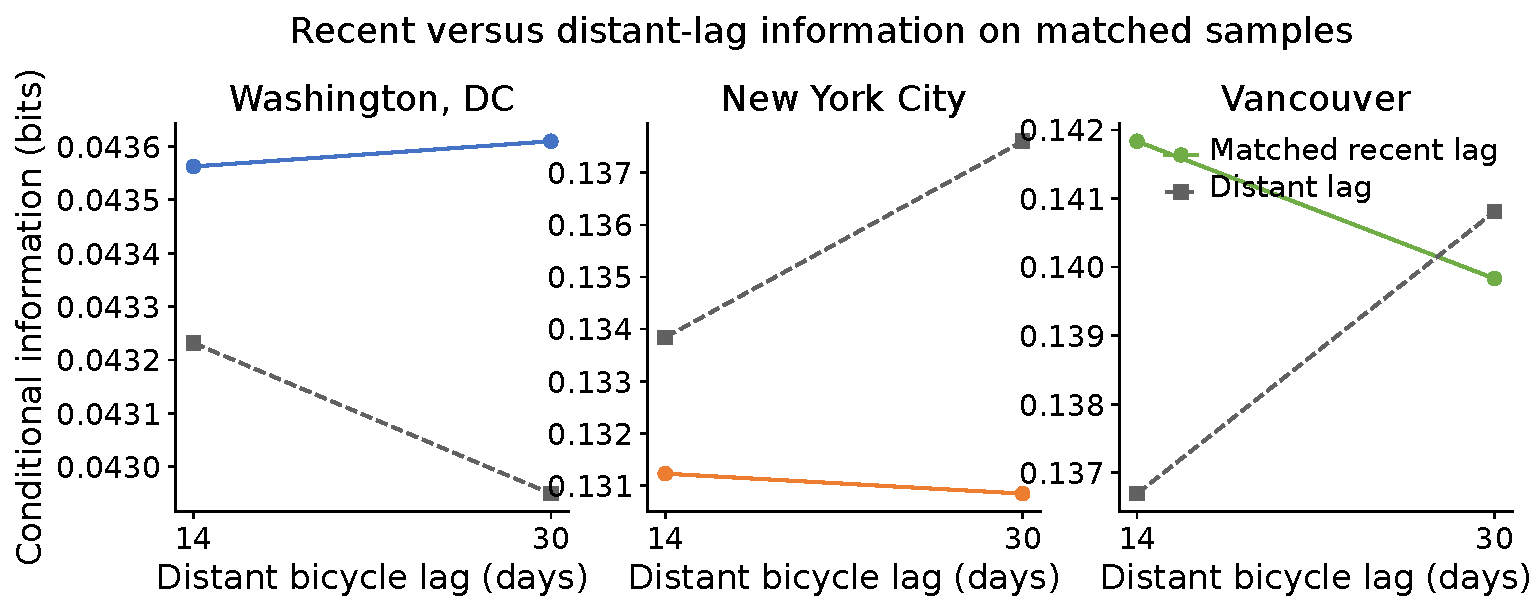
\includegraphics[width=\textwidth]{figures/e11/e10_distant_lags.pdf}
\caption{Matched recent- and distant-lag CMI estimates. Their similarity
shows that the positive primary point estimate is not specific to the
one-day mobility horizon.}
\label{fig:distant_lags}
\end{figure}

\section{Sample-Size and Multiscale Details}
\label{supsec:moved_scale}

\begin{table}[H]
\caption{Median relative deviation from the 100\% estimate across the 18 city--space--time cells. Quantiles over thinning repetitions are design-variability summaries, not population confidence intervals.}
\label{tab:e16_sample_stability}
\centering
\begin{tabular}{ccccc}
\toprule
\textbf{Sample fraction} & \textbf{Baseline DELB} & \textbf{Bicycle DELB} & \textbf{DELB reduction} & \textbf{CMI}\\
\midrule
20\% & 0.631 & 0.646 & 0.630 & 0.271\\
40\% & 0.423 & 0.448 & 0.341 & 0.250\\
60\% & 0.231 & 0.249 & 0.179 & 0.172\\
80\% & 0.101 & 0.114 & 0.070 & 0.087\\
100\% & 0.000 & 0.000 & 0.000 & 0.000\\
\bottomrule
\end{tabular}
\end{table}


\begin{figure}[!htbp]
\begin{adjustwidth}{-\extralength}{0cm}
\centering
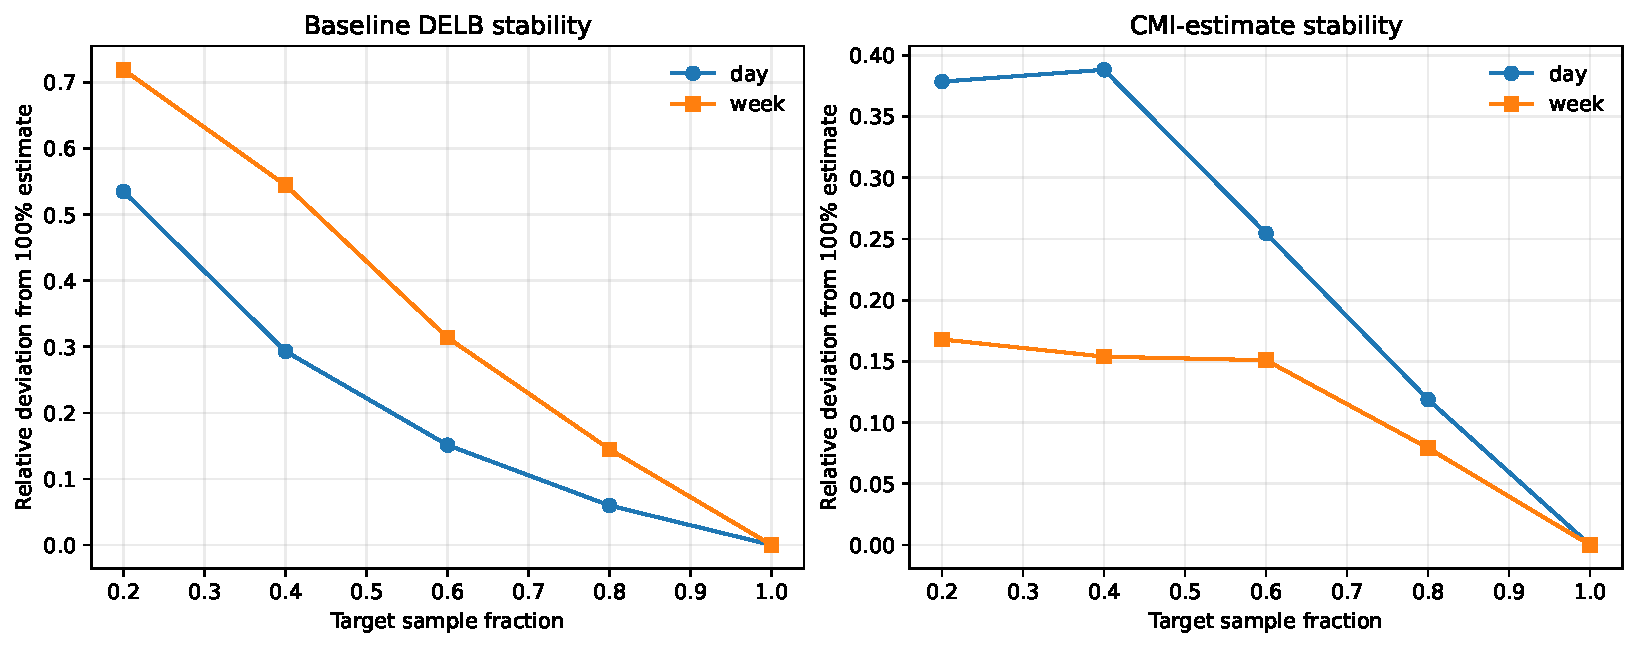
\includegraphics[width=\linewidth]{figures/e16/e16_s16_5_sample_stability.pdf}
\end{adjustwidth}
\caption{Relative deviation from the full-sample baseline DELB and CMI
estimate under nested block thinning. The curves measure estimator
stability, not distance from population truth.}
\label{fig:e16_sample_stability}
\end{figure}

\begin{figure}[!htbp]
\begin{adjustwidth}{-\extralength}{0cm}
\centering
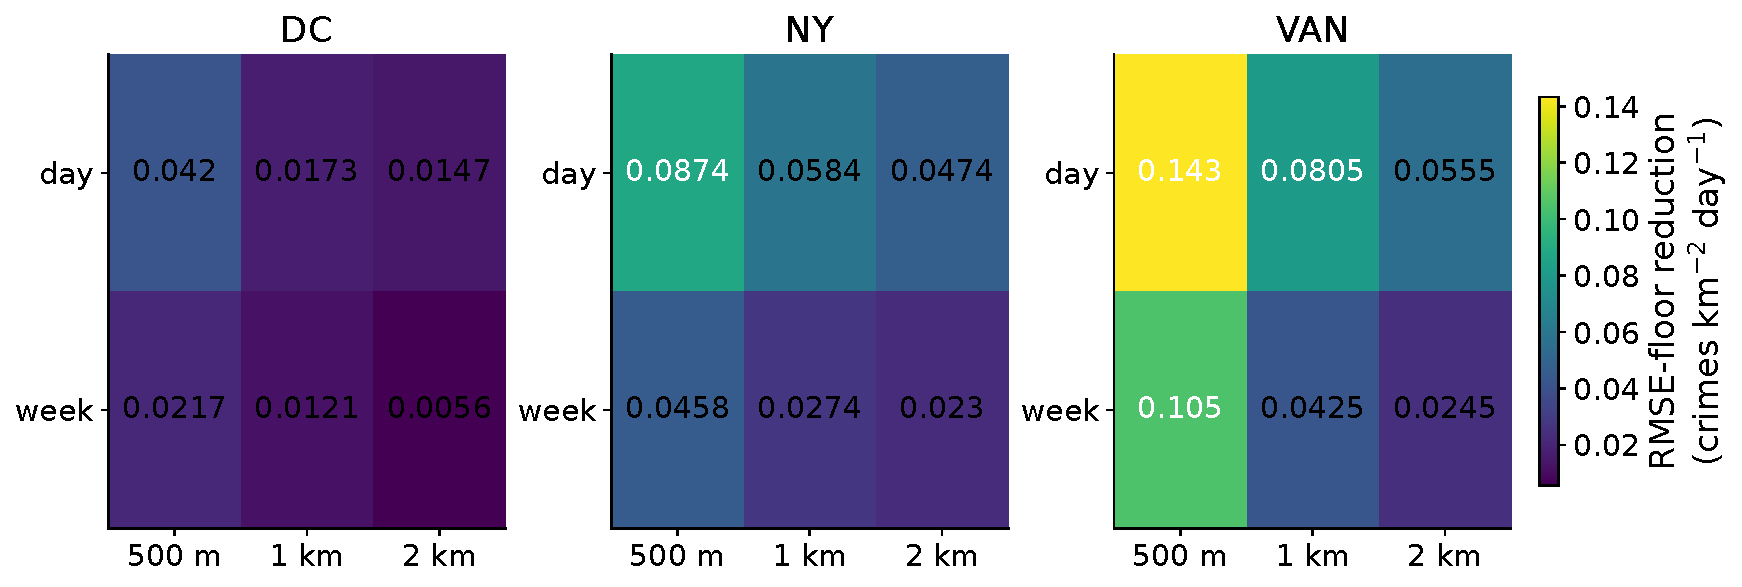
\includegraphics[width=\linewidth]{figures/e16/e16_s16_5_full_sample_intensity_heatmap.pdf}
\end{adjustwidth}
\caption{Full-sample Miller--Madow reduction in the deterministically scaled
intensity-RMSE floor by city, spatial resolution, and temporal resolution.}
\label{fig:e16_intensity_heatmap}
\end{figure}

\begin{figure}[!htbp]
\begin{adjustwidth}{-\extralength}{0cm}
\centering
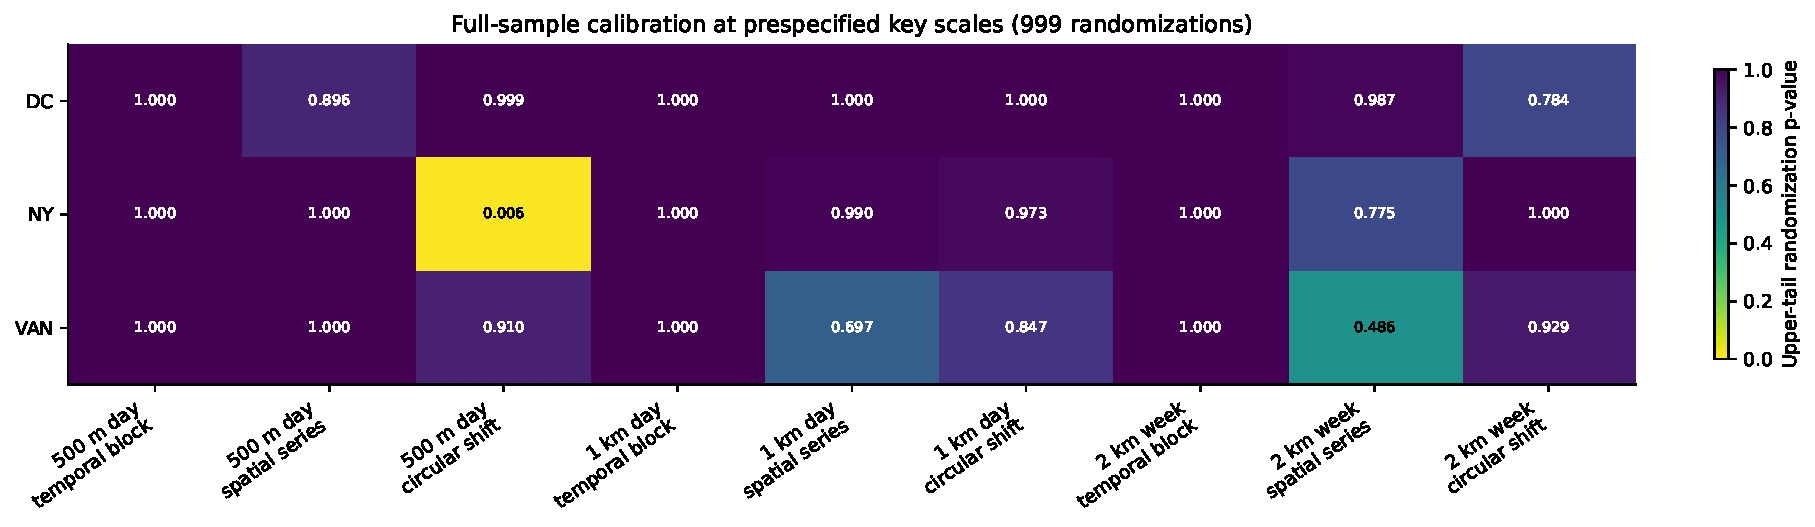
\includegraphics[width=\linewidth]{figures/e16/e16_s16_6_key_scale_pvalues.pdf}
\end{adjustwidth}
\caption{Full-sample upper-tail randomization \(p\)-values at the
500~m--day, 1~km--day, and 2~km--week key scales.}
\label{fig:e16_key_pvalues}
\end{figure}

\section{Crime-Type Heterogeneity}
\label{supsec:moved_crime_type}


\begin{table}[H]
\caption{Pooled crime-type heterogeneity in bicycle conditional information and DELB reduction. Intervals are centered 95\% seven-day block-bootstrap intervals for CMI.}
\label{tab:crime_type_heterogeneity}
\centering
\begin{tabular}{llrrrr}
\toprule
\textbf{City} & \textbf{Crime type} & \textbf{CMI} &
\textbf{95\% CI} & \(\boldsymbol{\Delta L}\) & \(\boldsymbol{R^L}\)\\
\midrule
Washington, DC & Property theft & 0.035 & [0.032, 0.038] & 0.009 & 7.1\%\\
Washington, DC & Vehicle theft & 0.012 & [0.011, 0.014] & 0.002 & 6.7\%\\
Washington, DC & Burglary & 0.006 & [0.005, 0.007] & 0.001 & 7.7\%\\
New York City & Property theft & 0.113 & [0.105, 0.121] & 0.045 & 15.8\%\\
New York City & Vehicle theft & 0.023 & [0.021, 0.025] & 0.004 & 10.1\%\\
New York City & Burglary & 0.028 & [0.026, 0.031] & 0.006 & 9.3\%\\
Vancouver & Property theft & 0.114 & [0.100, 0.128] & 0.060 & 14.9\%\\
Vancouver & Vehicle theft & 0.013 & [0.011, 0.015] & 0.002 & 8.1\%\\
Vancouver & Burglary & 0.041 & [0.034, 0.048] & 0.010 & 9.1\%\\
\bottomrule
\end{tabular}
\end{table}


\begin{figure}[!htbp]
\centering
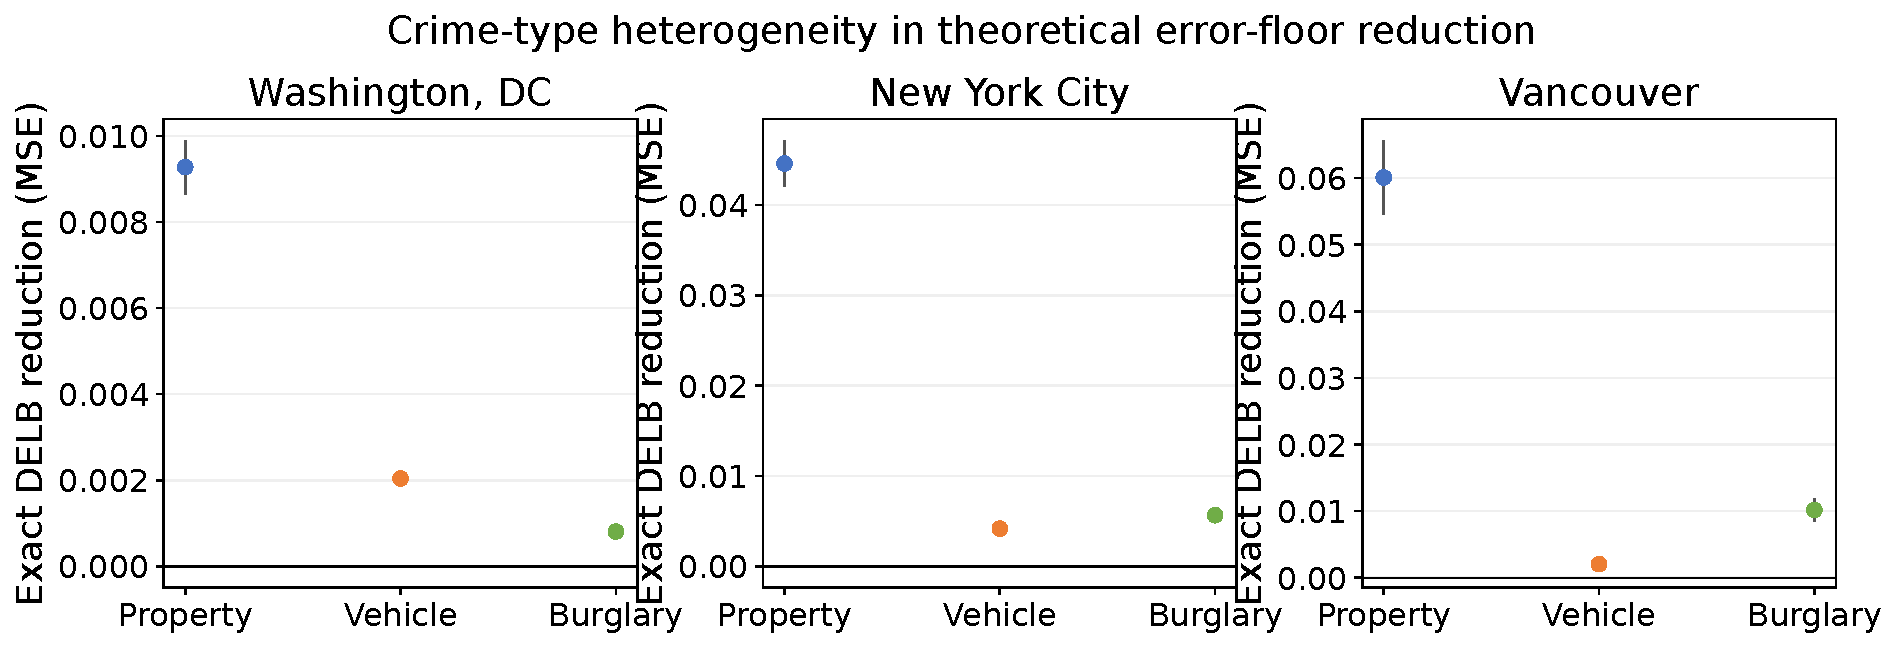
\includegraphics[width=\textwidth]{figures/e11/e08_crime_type_delb_reduction.pdf}
\caption{DELB-reduction point estimates by harmonized crime category and
city. Intervals measure block-bootstrap sampling variation and are not
category-specific randomization tests.}
\label{fig:crime_type_delb}
\end{figure}

\section{Alternative Specifications and Rolling Origins}
\label{supsec:moved_rolling}


\begin{table}[H]
\caption{Robustness summary across information specifications and rolling forecasts. Positive theory specifications count
Miller--Madow DELB reductions across 16 pre-specified alternatives.
Rolling forecasts comprise 12 monthly origins for each of four model
families. Positive \(\Delta\mathrm{MSE}\) favors the bicycle-aware model.}
\label{tab:robustness_summary}
\begin{adjustwidth}{-\extralength}{0cm}
\centering
\resizebox{\linewidth}{!}{%
\begin{tabular}{lrrrrrr}
\toprule
\textbf{City} & \textbf{Positive theory} & \textbf{Positive origins} &
\multicolumn{2}{c}{\textbf{State mean}} &
\multicolumn{2}{c}{\textbf{Gradient boosting}}\\
\cmidrule(lr){4-5}\cmidrule(lr){6-7}
 & & & \textbf{Positive} & \textbf{Mean \(\Delta\)MSE} &
\textbf{Positive} & \textbf{Mean \(\Delta\)MSE}\\
\midrule
Washington, DC & 16/16 & 23/48 & 66.7\% & 0.001 & 41.7\% & 0.000\\
New York City & 16/16 & 26/48 & 91.7\% & 0.030 & 100.0\% & 0.076\\
Vancouver & 16/16 & 20/48 & 66.7\% & 0.006 & 41.7\% & -0.006\\
\bottomrule
\end{tabular}
}
\end{adjustwidth}
\end{table}


\begin{figure}[!htbp]
\begin{adjustwidth}{-\extralength}{0cm}
\centering
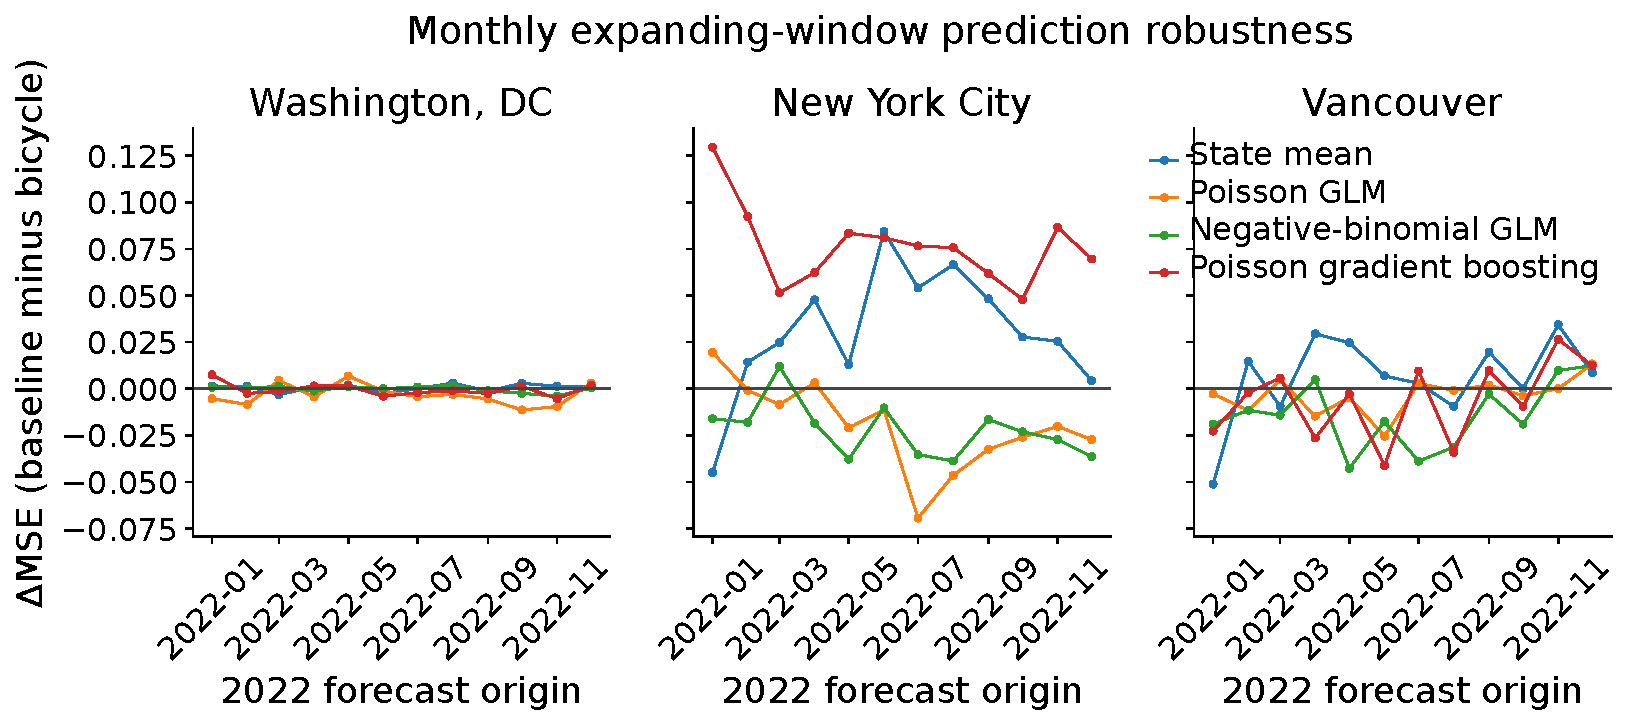
\includegraphics[width=\linewidth]{figures/e11/e09_rolling_origins.pdf}
\end{adjustwidth}
\caption{Expanding-window monthly prediction results. Positive
\(\Delta\mathrm{MSE}\) favors the bicycle-aware model; stability remains
model-specific.}
\label{fig:rolling_origins}
\end{figure}

\section{Additional Descriptive and Finite-Sample Figures}
\label{supsec:additional_figures}

Figures~\ref{fig:spatial_patterns} and \ref{fig:monthly_patterns} are
descriptive audits. They precede conditioning and are not evidence of CMI,
a DELB reduction, or a causal mobility effect.

\begin{figure}[!htbp]
\begin{adjustwidth}{-\extralength}{0cm}
\centering
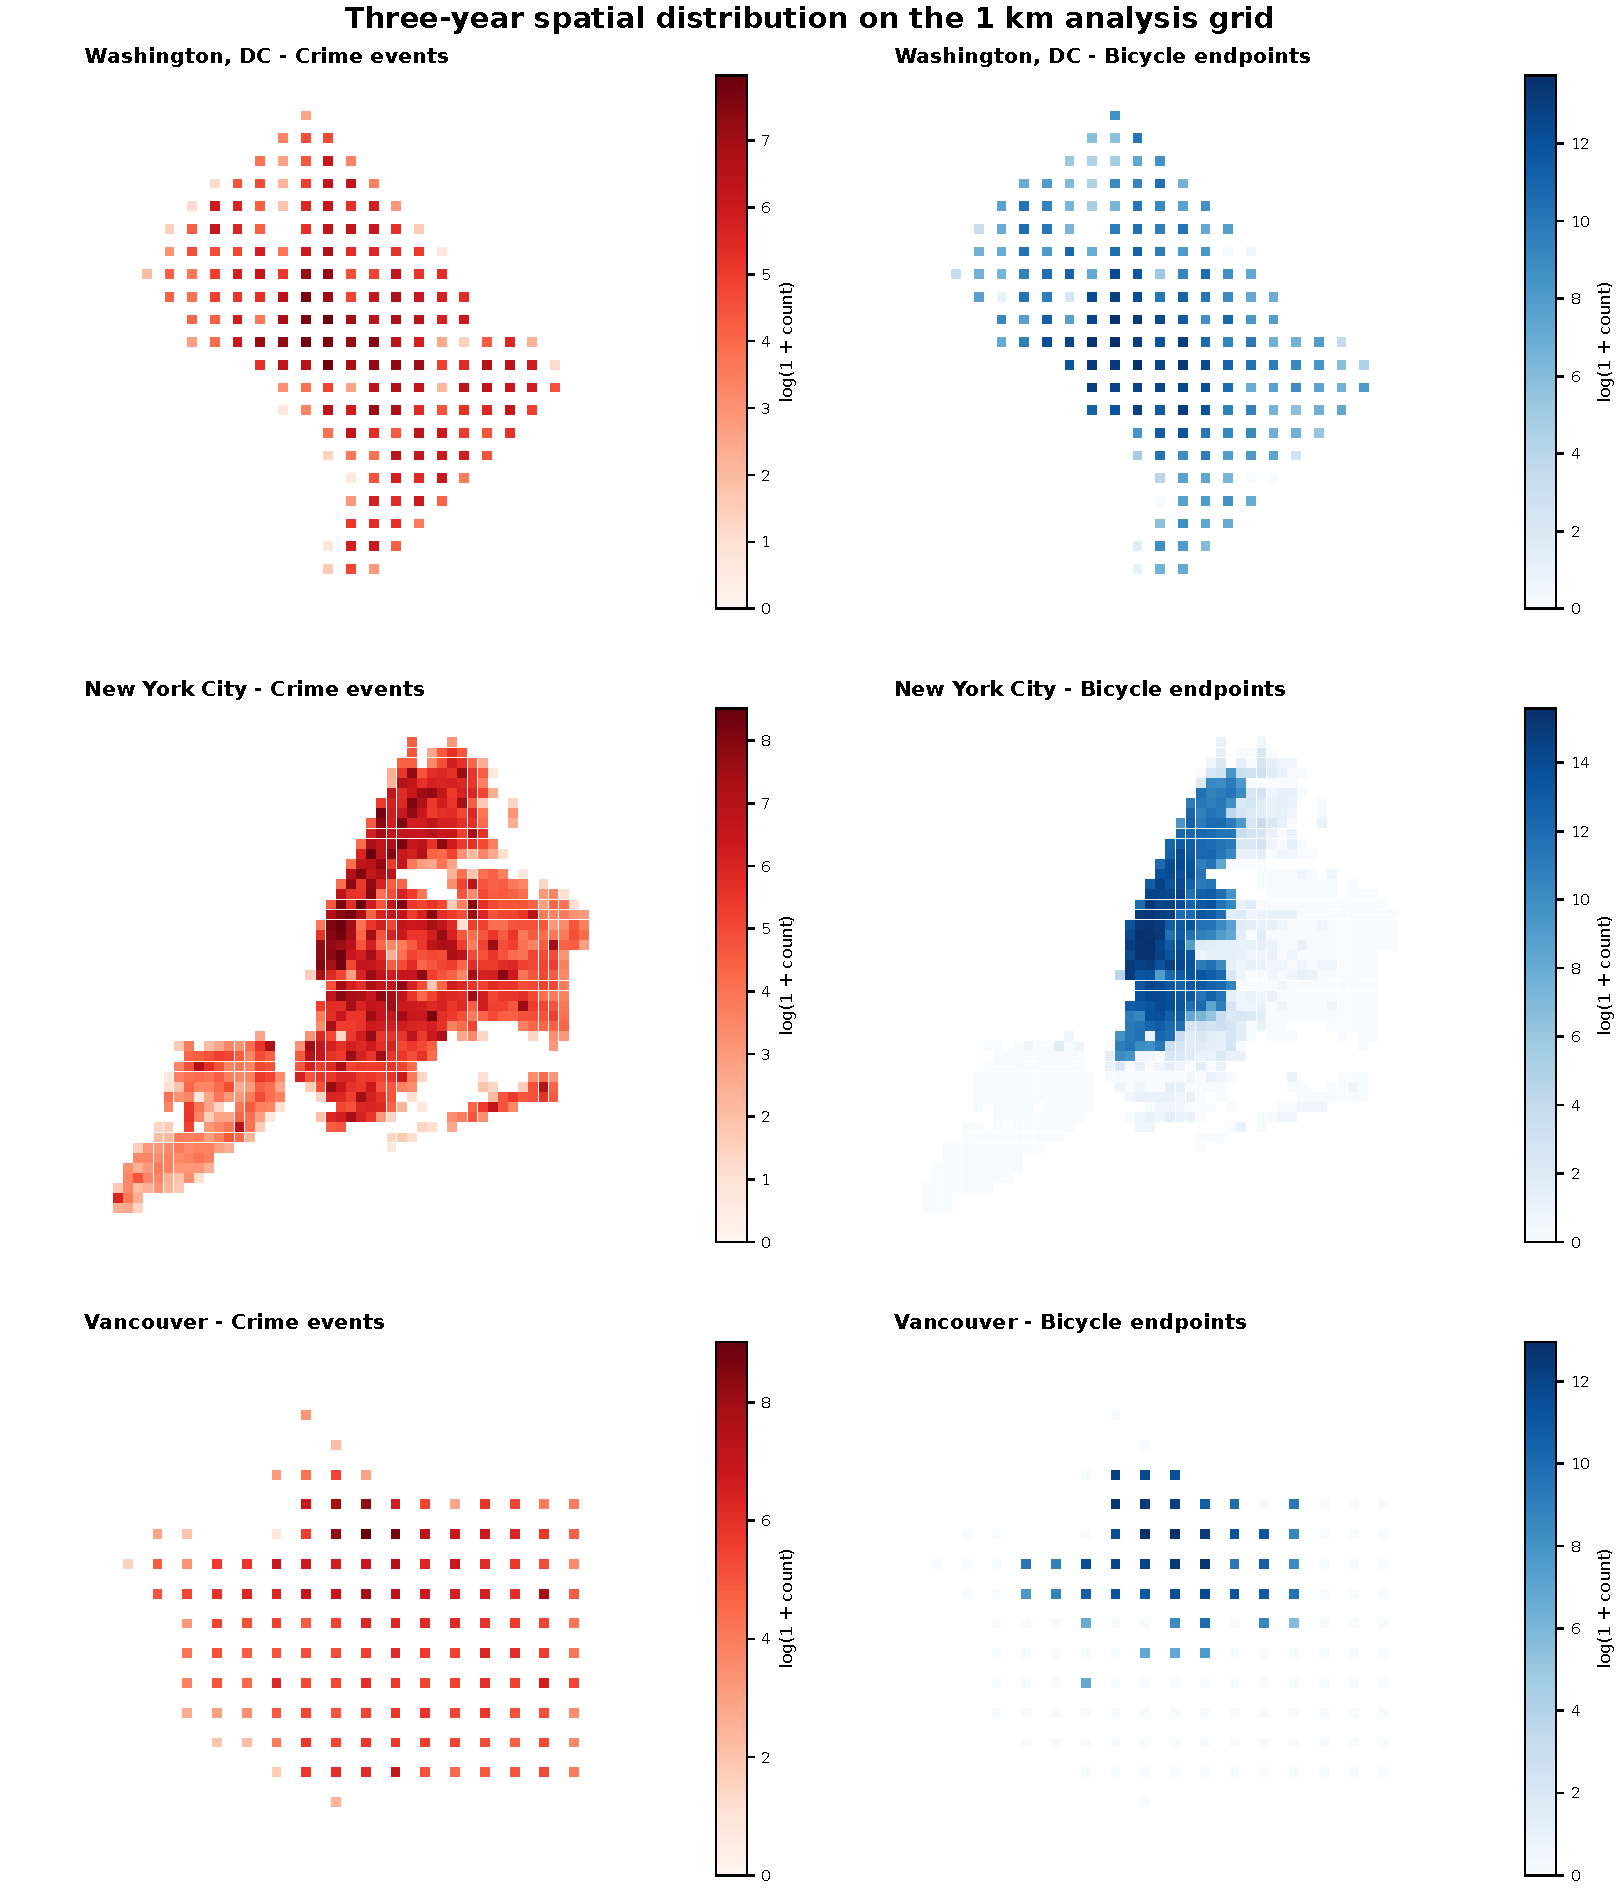
\includegraphics[width=0.98\linewidth]{figures/e11/e02_spatial_patterns.pdf}
\end{adjustwidth}
\caption{Spatial concentration of harmonized property-crime counts and
bicycle endpoint flow, 2020--2022.}
\label{fig:spatial_patterns}
\end{figure}

\begin{figure}[!htbp]
\centering
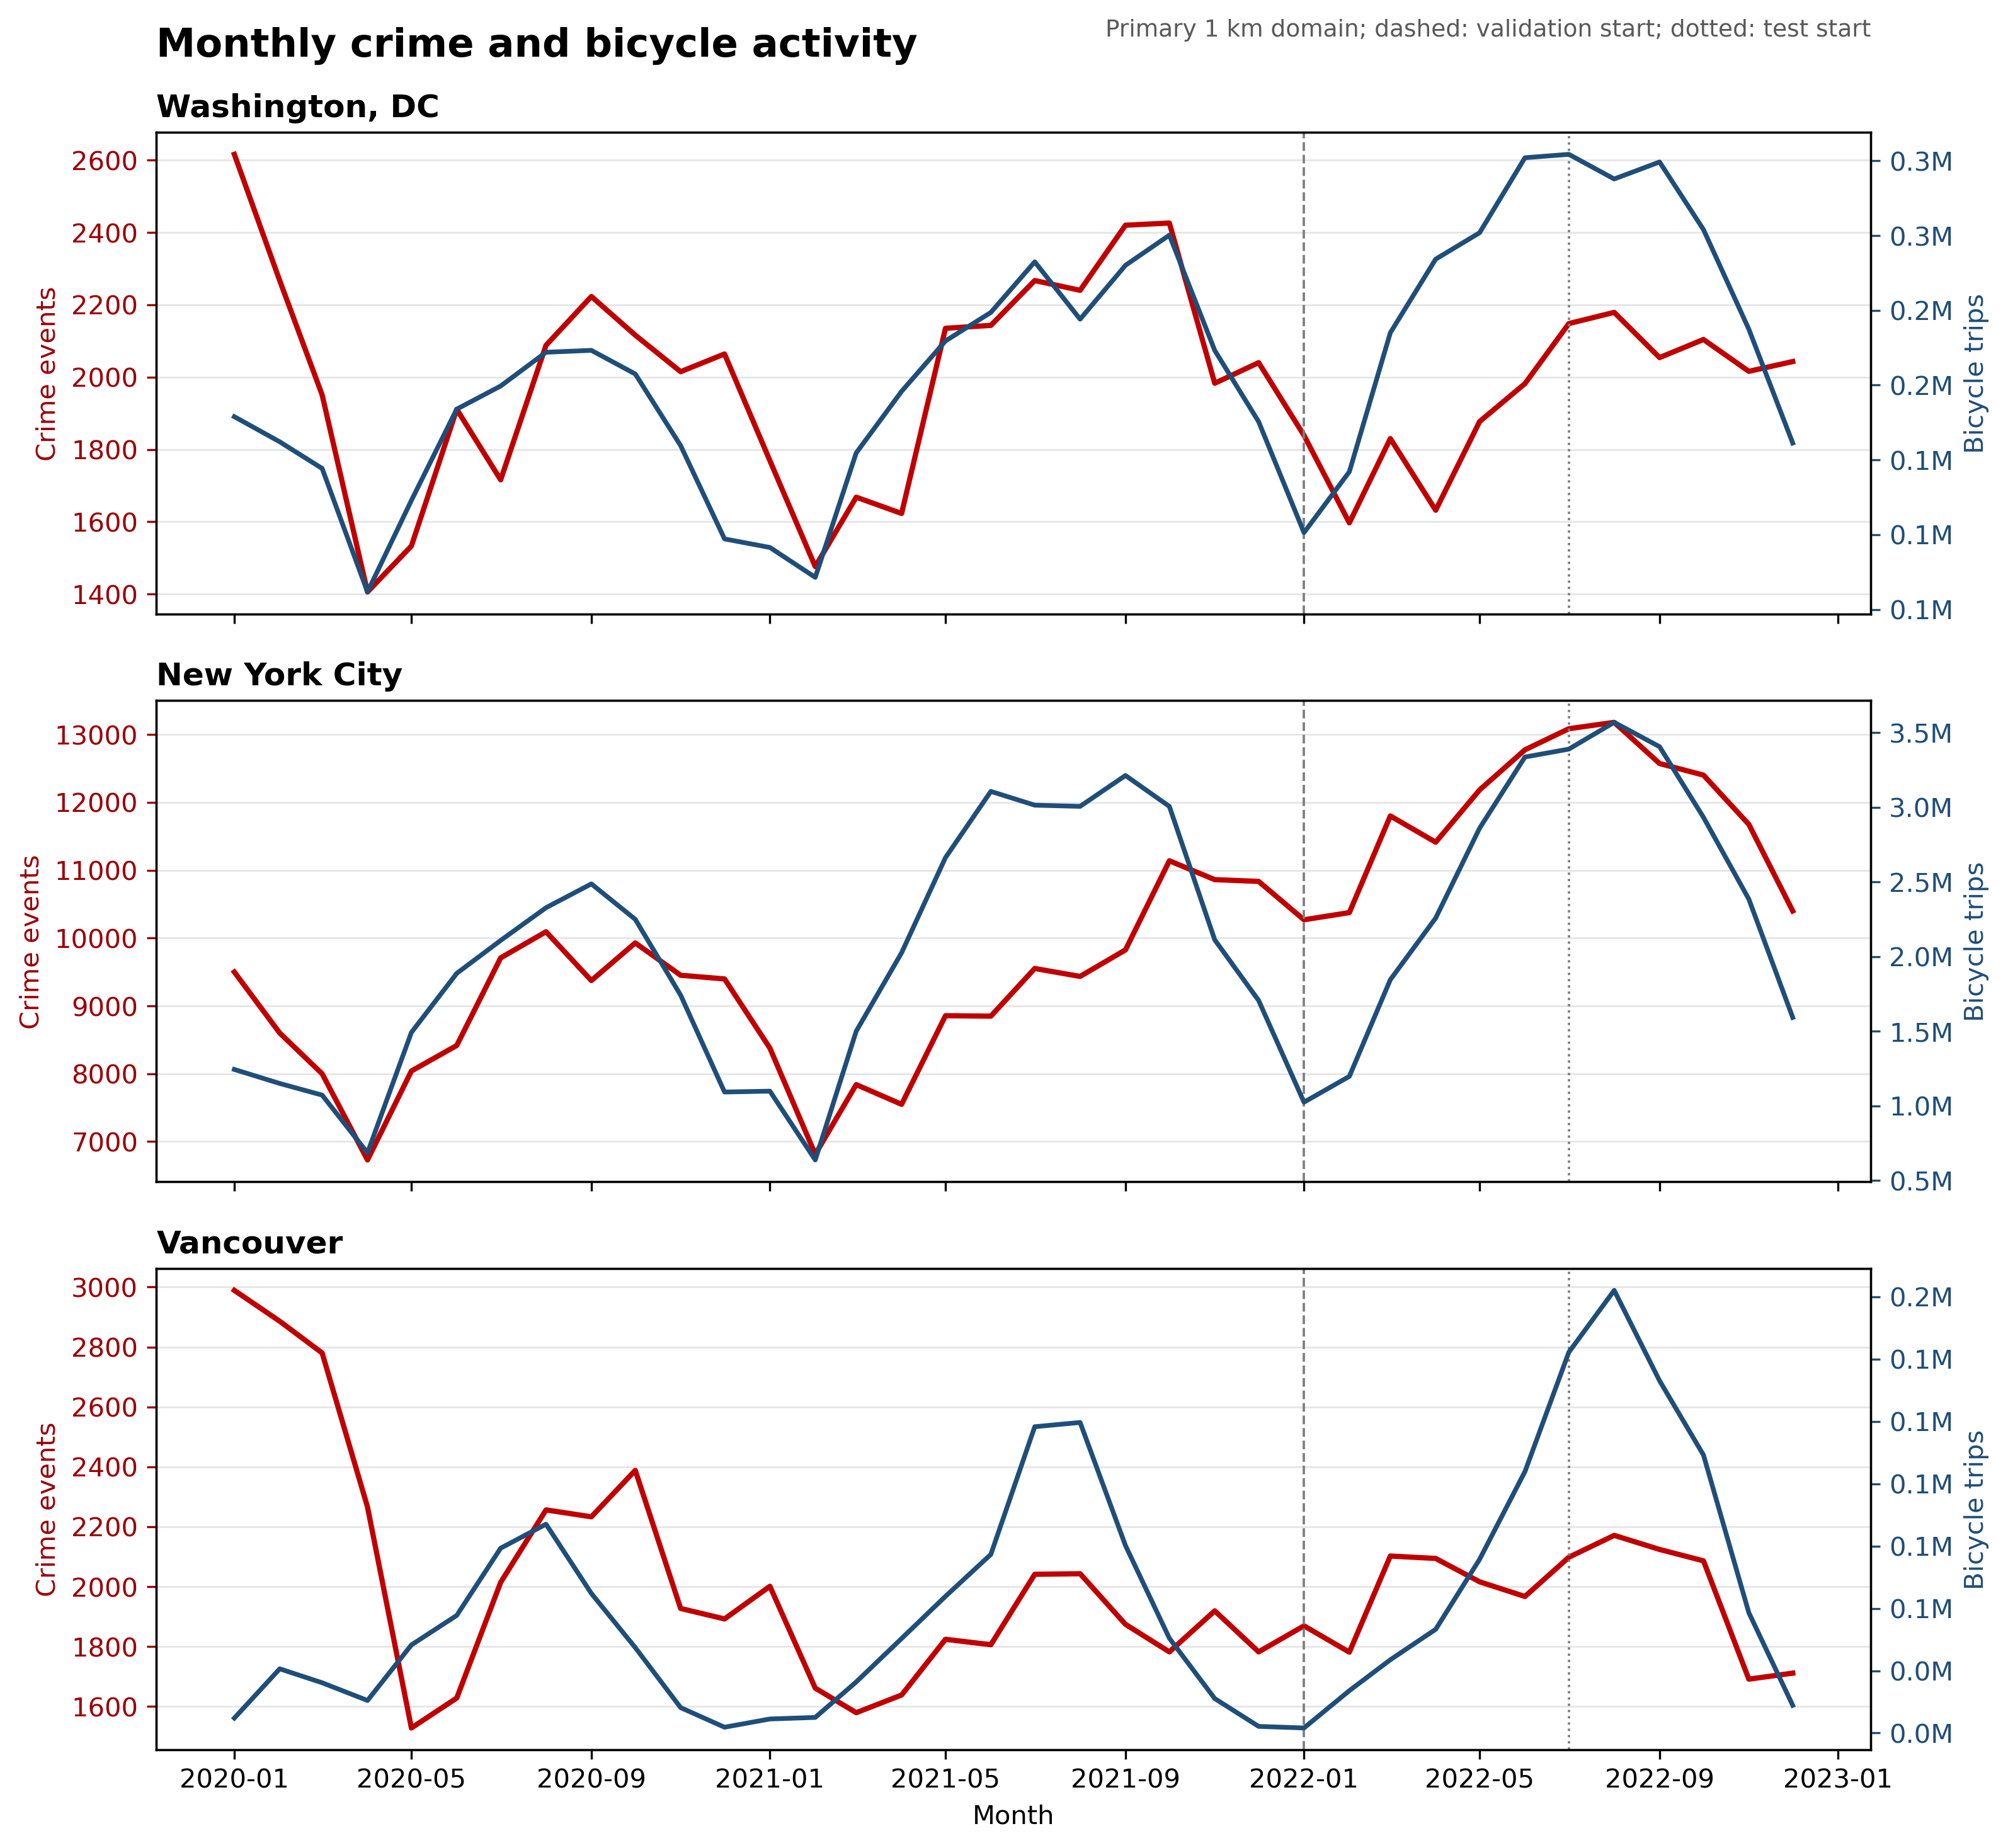
\includegraphics[width=\textwidth]{figures/e11/e02_monthly_patterns.png}
\caption{Monthly crime counts and bicycle endpoint flow by city,
2020--2022.}
\label{fig:monthly_patterns}
\end{figure}

\begin{figure}[!htbp]
\begin{adjustwidth}{-\extralength}{0cm}
\centering
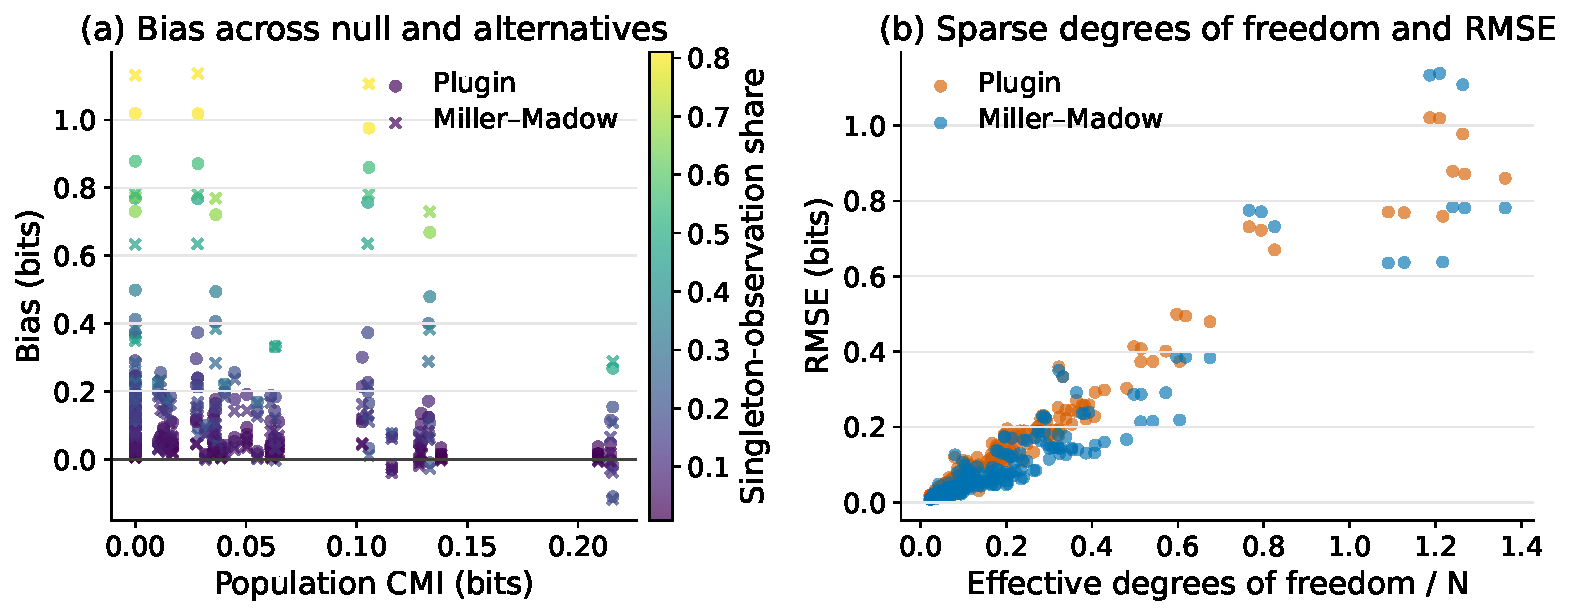
\includegraphics[width=\linewidth]{figures/s7/e12_bias_rmse_supplement.pdf}
\end{adjustwidth}
\caption{Estimator bias and RMSE over the complete sparse-state simulation
grid.}
\label{fig:e12_bias_supplement}
\end{figure}

\begin{figure}[!htbp]
\begin{adjustwidth}{-\extralength}{0cm}
\centering
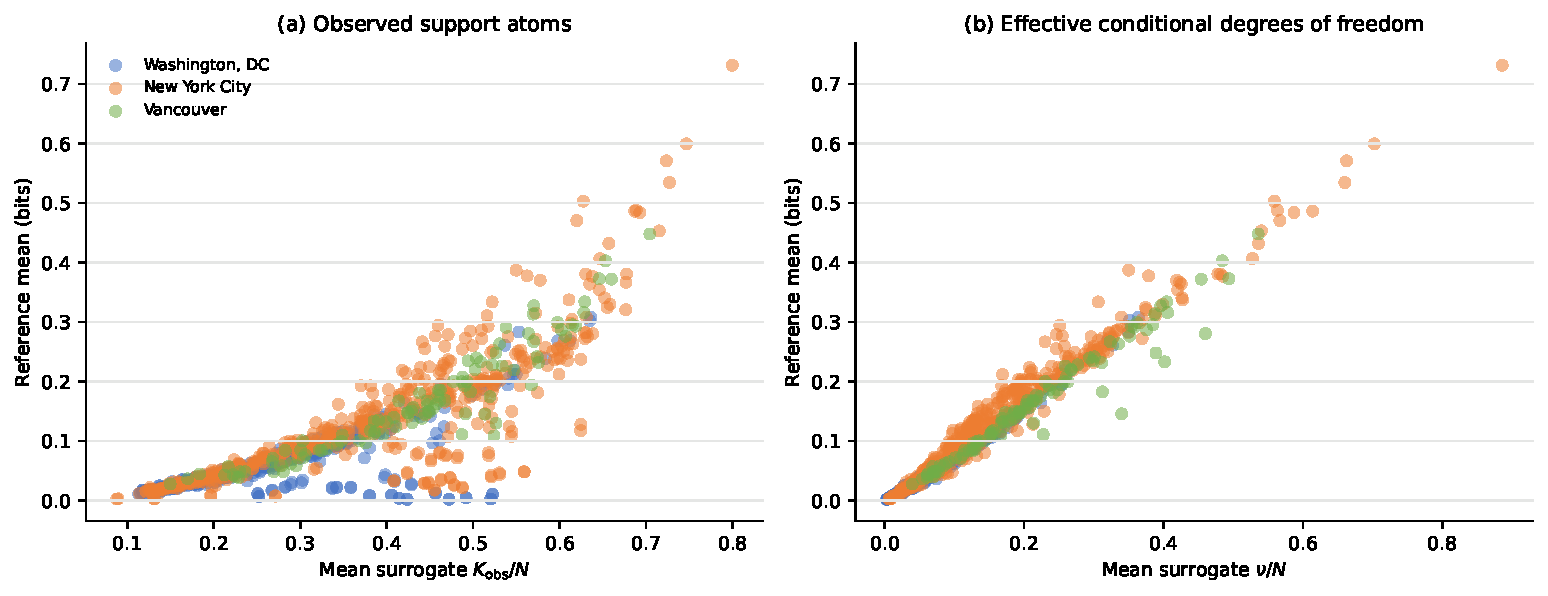
\includegraphics[width=\linewidth]{figures/s7/e13_support_metrics_supplement.pdf}
\end{adjustwidth}
\caption{Supplementary support-metric relationships for simulation and
empirical null summaries.}
\label{fig:e13_support_supplement}
\end{figure}

\begin{figure}[!htbp]
\begin{adjustwidth}{-\extralength}{0cm}
\centering
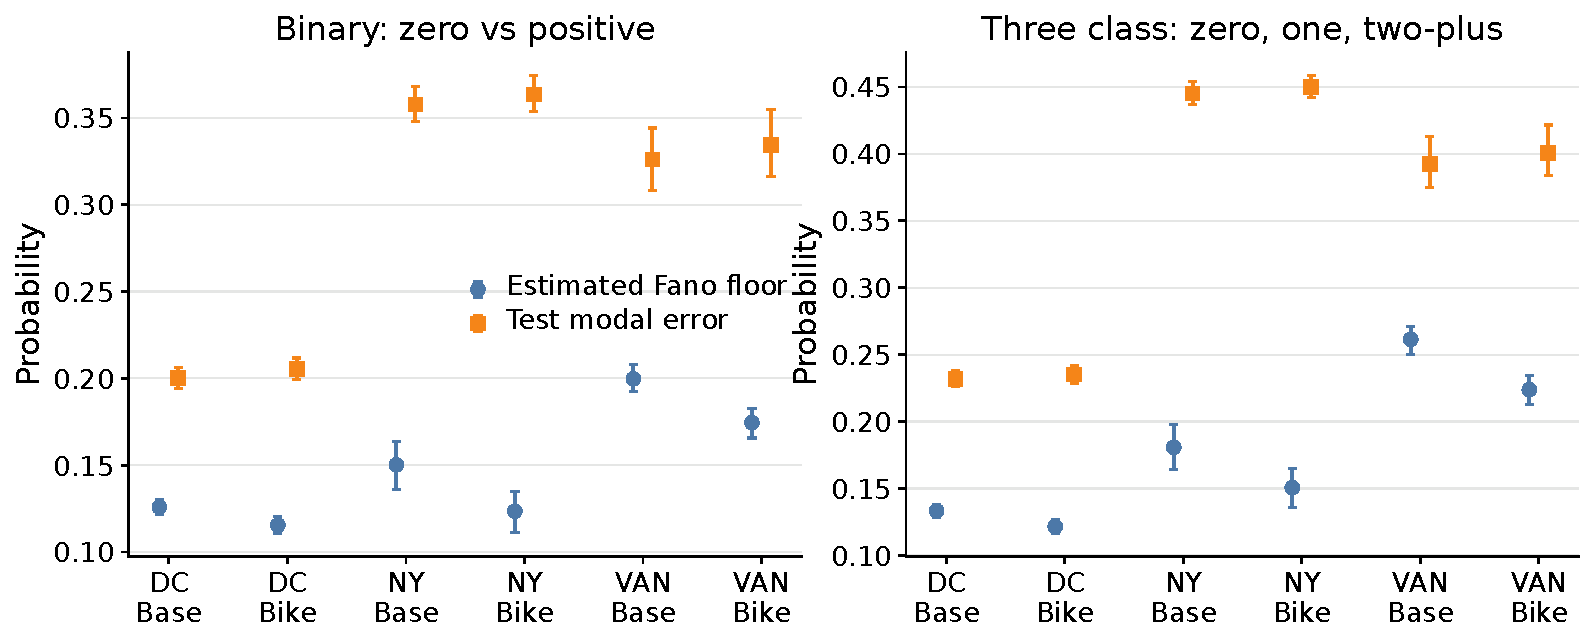
\includegraphics[width=\linewidth]{figures/s7/e14_fano_bootstrap.pdf}
\end{adjustwidth}
\caption{Centered seven-day block-bootstrap intervals for estimated Fano
floors and held-out modal-classifier errors.}
\label{fig:e14_bootstrap_supplement}
\end{figure}
